\documentclass[submission,copyright,creativecommons]{eptcs}
\providecommand{\event}{SOS 2007} % Name of the event you are submitting to
\usepackage{breakurl}             % Not needed if you use pdflatex only.
\usepackage{graphicx}
\usepackage{hyperref}
\usepackage{amsmath}
\usepackage{placeins}
\usepackage{float}
\usepackage{color}
\restylefloat{table}
\usepackage[belowskip=-15pt,aboveskip=0pt]{caption}

\title{Comparison of Machine Learning Algorithms For Intrusion Detection Tool}
\author{Sinan Talha KOŞAR
\institute{Computer Engineering}
\institute{Middle East Technical University\\ Ankara, Turkey}
\email{SN:2099190}
\email{e2099190@ceng.metu.edu.tr}
\and
Kenan Faruk Çakır
\institute{Computer Engineering}
\institute{Middle East Technical University\\ Ankara, Turkey}
\email{SN:2171445}
\email{e2171445@ceng.metu.edu.tr}
\and
Oğuzcan Budumlu
\institute{Computer Engineering}
\institute{Middle East Technical University\\ Ankara, Turkey}
\email{SN:2098820}
\email{e2098820@ceng.metu.edu.tr}
}

\begin{document}
\maketitle 

\begin{abstract}
\textbf{\textit{Abstract--}IDS is an acronym for “Intrusion Detection System”, a device or application used to inspect all network traffic and alert the user or administrator when there has been unauthorized attempts or access. We have implemented some machine learning classifiers into our intrusion database and compared the results.\\
\\
\textit{Index Terms--}Intrusion Detection, IDS, Attacker, Network, Machine Learning, Neural Network, Bayesian Neural Network, Decision Tree, Adaboost, Random Forest, Naive Bayes, Multi-Layer Perceptron}
\end{abstract}

\section{Introduction}
No firewall is foolproof, and no impenetrable network\cite{b1}.
Attackers finding new vulnerabilities and attacking techniques nonstop to bypass systems defenses. An intrusion detection system (IDS) is crucial for network protection by listening and detecting malicious traffic. From an intrusion detection perspective, analysts can apply machine learning algorithms to distinguish between normal and malicious traffic. In this research many machine learning algorithms implementation over intrusion detection datasets will be compared. In this research, signature-based intrusion detection implemented.

\section{Problem statement}
An intrusion detection system (IDS) monitors the network to detect malicious traffic. Traditional systems were designed to detect known attacks but cannot identify unknown threats. Their process based on defined rules. Nowadays attackers can bypass these traditional systems, so the need for more intelligent intrusion detection is increasing by the day. Researchers are attempting to apply machine learning techniques to this area of cybersecurity. There are lots of machine learning algorithms and models available each has advantages and disadvantages.
We aim to categorize and compare some machine learning algorithms we will mention below according to how well they perform on different types of numerous security attacks. In different scenarios, different type of attacks , machine learning algorithms reliability differ. We will demonstrate which machine learning algorithms perform better and worse in certain cases using precision, recall, accuracy and F-1 scores measures, also plots.\cite{b5}\\
\newpage
Machine Learning Algorithms We Have Used:
\begin{itemize}
  \item Decision Tree Classifier
  \item Adaboost Classifier
  \item Random Forest Classifier
  \item Naive Bayes Network
  \item Multi-Layer Perceptron
\end{itemize}

Security Attacks We Have Classified Using Above Algorithms:
\begin{itemize}
    \item Brute Force
    \item FTP-Patator
    \item SSH-Patator
    \item DoS / DDoS
    \item Heartbleed Port 444
    \item Web Attack – Brute Force
    \item Web Attack – XSS
    \item Web Attack – SQL Injection
    \item Infiltration
    \item Botnet

\end{itemize}


\section{Related Works}

Many Network based Intrusion Detection Systems use machine learning these days with the emergence of Big Data, many researches use machine learning to establish high speed and accurate intrusion detection systems. Machine learning (ML) is used for network intrusion detection because of its prediction ability after training with relevant data. ML provides a good method to detect new and unknown attacks. There are available security tools such as network intrusion detection and prevention systems to spot intruders before they can do serious damage. Here some of the examples of intrusion prevention systems.\\
\\
\textbf{McAfee NSP}

The McAfee Network Security Platform (NSP) is an intrusion prevention solution that protects systems across data centers, the cloud, and etc. It can support up to 32 million connections on a single appliance.\cite{b2}\\
\\
\textbf{Cisco Firepower NGIPS}

Cisco's Next-Generation Intrusion Prevention System comes in software, physical and virtual appliances for small offices to large companies. Product offers URL-based security intelligence, AMP Threat Grid integration.\cite{b2}
\subsection{References}
\begin{itemize}
    \item Phadke, A., Kulkarni, M., Bhawalkar, P., \& Bhattad, R. (2019). A Review of Machine Learning Methodologies for Network Intrusion Detection. 2019 3rd International Conference on Computing Methodologies and Communication (ICCMC), 272-275.
    \item Kok, S., Abdullah, A., Supramaniam, M., Pillai, T.R., \& Hashem, I.A. (2019). A Comparison of Various Machine Learning Algorithms in a Distributed Denial of Service Intrusion.
    \item Biswas, S.K. (2018). Intrusion Detection Using Machine Learning: A Comparison Study.
    \item Robb, D. (n.d.). Guide to IDPS. Retrieved June 28, 2020, from https://www.esecurityplanet.com/products/top-intrusion-detection-prevention-systems.html

\end{itemize}
\section{Proposed Approach}
There are two different approaches applied. One of them is preprocessing each dataset before fitting them into models then classifying each concurently and other one is concatenating all datasets then making preprocessing before classifying as one piece.
The following steps are the same for both modes.
\begin{enumerate}
\setcounter{enumi}{-1}
\item \textbf{Read dataset}\\
The datasets in CSV format are read and they are kept in DataFrame format. All steps after this will be done on DataFrames but however they are referred as datasets. During read operation, duplicate columns are reduced to one column as well.
\item \textbf{Data preprocessing}\\
Dataset is preprocessed for feature selection.
\begin{enumerate}
    \item[1.1] \textbf{Dataset Normalization}\\
    Dataset is normalized. All features are made numerical.
    \item[1.2] \textbf{Dataset Split}\\
    The dataset is split so that 80 percent of it is train dataset and 20 percent is test dataset. 
    \item[1.3] \textbf{Label Replace}\\
    Labels are enumerated in splitted datasets.
    \item[1.4] \textbf{Obtain Feature and Label Datasets}\\
    While feature dataset is obtained by dropping label dataset in train and test datasets, label datasets is obtained by dropping feature dataset in train and test datasets.
    \item[1.5] \textbf{Clean Datasets}\\
    NaN, INF, -INF values are removed from the most recently removed datasets.
\end{enumerate}
\newpage
\item \textbf{Feature selection}\\
The main purpose is that features which represent the attacks are selected. Irrelevant and redundant features are eliminated. The models are trained with selected features. We have plotted the number of selected features and cross validation score to validate the number of selected features of our algorithm. We have seen that the results are same.
\begin{figure}[H]
\centerline{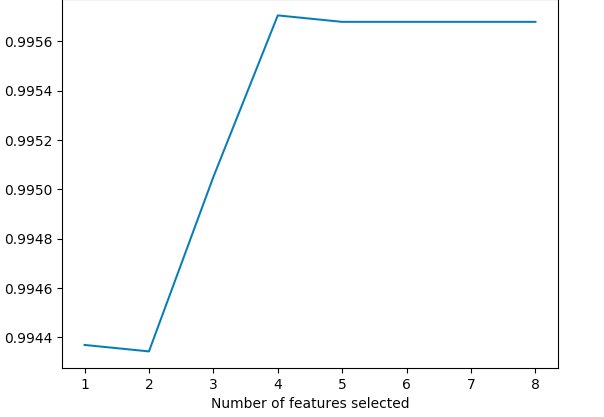
\includegraphics[height=8cm,width=10cm]{fs.png}}
\caption{Feature Selection}
\end{figure}
\begin{enumerate}
    \item[2.1] \textbf{Scaling}\\
    Before selecting the features, train and test feature datasets are scaled with SelectPercentile. It transforms the datasets such that distribution of them has mean of 0 and standard deviation of 1.
    \item[2.2] \textbf{Univariate feature selection}\\
    Each feature is analyzed by comparing with a target variable. When it is the case, other features are ignored so that’s why it is called ‘univariate’. For this purpose, f\_classif parameter is used in feature selector.
    \item[2.3] \textbf{Feature Selection}\\
    Giving “percent of features to keep” as 10 and f\_classif as parameters to SelectPercentile, feature selection model is built. Then, selected features are obtained with label dataset and scaled feature dataset.

\end{enumerate}
\item \textbf{Build model}\\
For building, Decision Tree, Adaboost, Random Forest models, Naive Bayes Network and Multi-Layer Perceptron are used.  
\item \textbf{Prediction and Evaluation}\\
After building the model, prediction is made with the test feature dataset and evaluation is made by comparing the prediction dataset and test label dataset.
\end{enumerate}

\begin{figure}[h]
\centerline{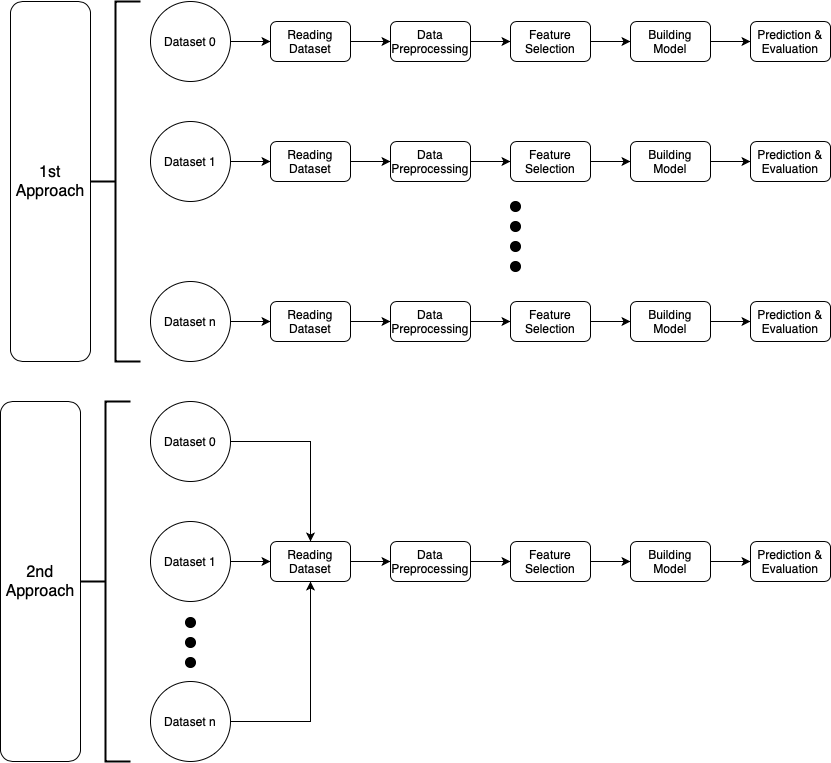
\includegraphics[height=10cm,width=15cm]{approaches.png}}
\caption{Approaches Flow Chart}
\end{figure}

\section{Experiment results}
In the tables below, row numbers represent different datasets we used to train and test our models.\\
Used datasets to train and test our different models can be seen at link: \\
\begin{itemize}
    \item \href{https://www.unb.ca/cic/datasets/ids-2017.html}{IDS 2017 | Datasets | Research | Canadian Institute for Cybersecurity}.\\
\end{itemize}
\textbf{Mapping of row numbers and datasets:}
\begin{enumerate}
\setcounter{enumi}{-1}
    \item Thursday-WorkingHours-Afternoon-Infilteration.pcap\_ISCX.csv
    \item Wednesday-workingHours.pcap\_ISCX.csv
    \item Friday-WorkingHours-Afternoon-DDos.pcap\_ISCX.csv
    \item Monday-WorkingHours.pcap\_ISCX.csv
    \item Thursday-WorkingHours-Morning-WebAttacks.pcap\_ISCX.csv
    \item Tuesday-WorkingHours.pcap\_ISCX.csv
    \item Friday-WorkingHours-Afternoon-PortScan.pcap\_ISCX.csv
    \item Friday-WorkingHours-Morning.pcap\_ISCX.csv

\end{enumerate}
* Notice that in below result tables row 3 is omitted. It is because in that dataset, there was no attack, all data was benign, therefore feature selection was not possible.\\

Ps. After doing some research we have conclude that if dataset labels are not uniform then accuracy will no longer be meaningful.

\subsection{Decision Tree Classifier}
In decision tree no need for normalization and scaling and missing values not affect the process, so this make one of our choices is decision tree. We have seen that the decision tree model is consistent in its accuracy values when run multiple times. In datasets 2 and 6, it has a little low accuracy. Also, decision tree often involves higher time to train the model and no need for normalizing and scaling dataset, therefore we haven't done any normalization or scaling to save time.
\\
\begin{figure}[h!]
\begin{minipage}{.3\linewidth}
    \centering
    \[\left[\begin{array}{cccc}
      87509 & 57 & 273 & 0\\
      267 & 1712 & 53 & 0\\
      1561 & 99 & 32616 & 0\\
      0 & 1 & 0 & 0\\
    \end{array}\right]\]
    Dataset\_1 CM
  \end{minipage} 
  \begin{minipage}{.15\linewidth}
    \centering
    \[\left[\begin{array}{cc}
      105883
    \end{array}\right]\]
    Dataset\_3 CM
  \end{minipage}%
  \begin{minipage}{.25\linewidth}
    \centering
    \[\left[\begin{array}{cccc}
      33233 & 259 & 88 & 2 \\
      315 & 0 & 0 & 0 \\
      133 & 0 & 0 & 0 \\
      6 & 0 & 0 & 0
    \end{array}\right]\]
    Dataset\_4 CM
  \end{minipage} 
  \begin{minipage}{.2\linewidth}
    \centering
    \[\left[\begin{array}{cc}
      37730 & 83 \\
      367 & 6
    \end{array}\right]\]
    Dataset\_7 CM
  \end{minipage}

  
  \caption{Some of confusion matrices(CM)}
\end{figure}\\
\begin{table}[h!]
\begin{center}
\begin{tabular}{|l|l|l|l|l|}
\hline
\textbf{Dataset}  & \textbf{Accuracy} & \textbf{Precision} & \textbf{Recall} & \textbf{F1 Score} \\ \hline
\textbf{0} & 0.999             & 0.999              & 0.999           & 0.999             \\ \hline
\textbf{1} & 0.881             & 0.897              & 0.881           & 0.874             \\ \hline
\textbf{2} & 0.794             & 0.860              & 0.794           & 0.791             \\ \hline
\textbf{4} & 0.976             & 0.973              & 0.976           & 0.974             \\ \hline
\textbf{5} & 0.962             & 0.937              & 0.962           & 0.949             \\ \hline
\textbf{6} & 0.723             & 0.827              & 0.723           & 0.710             \\ \hline
\textbf{7} & 0.988             & 0.981              & 0.988           & 0.984             \\ \hline
\end{tabular}
\caption{Decision Tree Classifier Scores}
\label{tab:my-table}
\end{center}
\end{table}
Datasets with surplus labels (dataset\_1) and datasets having less "BENIGN" as label have less scores compared to the others.
\subsection{Adaboost Classifier}
There are 2 different result tables below for the adaboost algorithm. We noticed in Datasets 1 and 6 , there is a flipping behaviour, and low measure values in dataset 2. This flipping behaviour is caused by the random selection of train and test data. If the dataset is not uniformly distributed, there is a possibility that the same labels fall into the same section.
\begin{table}[H]
\begin{center}
\begin{tabular}{|l|l|l|l|l|}
\hline
\textbf{Dataset}  & \textbf{Accuracy} & \textbf{Precision} & \textbf{Recall} & \textbf{F1 Score} \\ \hline
\textbf{0} & 0.999             & 0.999              & 0.999           & 0.999             \\ \hline
\textbf{1} & 0.742             & 0.847              & 0.742           & 0.781             \\ \hline
\textbf{2} & 0.639             & 0.802              & 0.639           & 0.607             \\ \hline
\textbf{4} & 0.949             & 0.973              & 0.949           & 0.961             \\ \hline
\textbf{5} & 0.968             & 0.938              & 0.968           & 0.953             \\ \hline
\textbf{6} & 0.002             & 0.003              & 0.002           & 0.003             \\ \hline
\textbf{7} & 0.995             & 0.995              & 0.995           & 0.995             \\ \hline
\end{tabular}
\caption{Adaboost Classifier Scores - 1}
\label{tab:my-table}
\end{center}
\end{table}
\begin{table}[H]
\begin{center}
\begin{tabular}{|l|l|l|l|l|}
\hline
\textbf{Dataset}  & \textbf{Accuracy} & \textbf{Precision} & \textbf{Recall} & \textbf{F1 Score} \\ \hline
\textbf{0} & 0.999             & 0.999              & 0.999           & 0.999             \\ \hline
\textbf{1} & 0.046             & 0.094              & 0.046           & 0.056             \\ \hline
\textbf{2} & 0.390             & 0.268              & 0.390           & 0.317             \\ \hline
\textbf{4} & 0.817             & 0.988              & 0.817           & 0.890             \\ \hline
\textbf{5} & 0.969             & 0.939              & 0.969           & 0.954             \\ \hline
\textbf{6} & 0.997             & 0.997              & 0.997           & 0.997             \\ \hline
\textbf{7} & 0.995             & 0.995              & 0.995           & 0.995             \\ \hline
\end{tabular}
\caption{Adaboost Classifier Scores - 2}
\label{tab:my-table}
\end{center}
\end{table}
Datasets with surplus labels (dataset\_1) and datasets having less "BENIGN" as label have less scores compared to the others.
\subsection{Random Forest Classifier}
We have chosen random forest classifier because there are lots of implementations on intrusion detection tool, so including it in project will be meaningful. Random forest has lots of decision trees. Low classification error compared to other algorithms. Although, it provides some feature selection we decided to use our feature selection algorithm to make comparison between classifier more accurate.
\begin{figure}[H]
\centerline{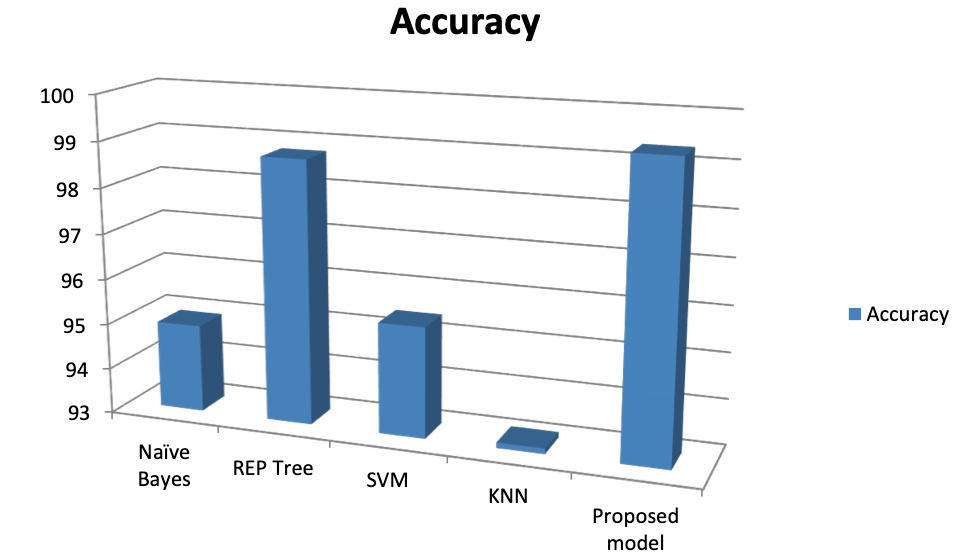
\includegraphics[height=10cm,width=10cm]{randomvs.png}}
\caption{Performance accuracy of proposed model and existing models, Reprinted from "Hadi, A. A. (2018). Performance Analysis of Big Data Intrusion Detection System over Random Forest Algorithm."\cite{b6}}
\captionsetup{belowskip=0pt}
\end{figure}
Ps. In above graph proposed model is random forest, the cited article is about comparing other models with random forest.
\begin{figure}[h!]
\begin{minipage}{.2\linewidth}
    \centering
    \[\left[\begin{array}{cc}
      57668 & 0\\
      4 & 3\\
    \end{array}\right]\]
    Dataset\_0 CM
  \end{minipage} 
  \begin{minipage}{.2\linewidth}
    \centering
    \[\left[\begin{array}{cc}
      25333 & 12\\
      110 & 31765\\
    \end{array}\right]\]
    Dataset\_6 CM
  \end{minipage} 
  \begin{minipage}{.2\linewidth}
    \centering
    \[\left[\begin{array}{cc}
      0 & 0\\
      19345 & 25801\\
    \end{array}\right]\]
    Dataset\_2 CM
  \end{minipage}
  \begin{minipage}{.2\linewidth}
    \centering
    \[\left[\begin{array}{ccc}
      86257 & 0 & 206\\
      0 & 0 & 0 \\
      2654 & 4 & 0\\
    \end{array}\right]\]
    Dataset\_5 CM
  \end{minipage} 
  \\
  \begin{minipage}{.3\linewidth}
    \centering
    \[\left[\begin{array}{cccc}
      33463 & 1 & 116 & 2\\
      315 & 0 & 0 & 0 \\
      133 & 0 & 0 & 0\\
      6 & 0 & 0 & 0\\
    \end{array}\right]\]
    Dataset\_4 CM
  \end{minipage}
  \begin{minipage}{.2\linewidth}
    \centering
    \[\left[\begin{array}{cc}
      37736 & 77\\
      262 & 111 \\
    \end{array}\right]\]
    Dataset\_7 CM
  \end{minipage}
  \begin{minipage}{.2\linewidth}
    \centering
    \[\left[\begin{array}{cccc}
      87721 & 49 & 69 & 0\\
      264 & 1733 & 35 & 0\\
      15253 & 105 & 33028 & 0\\
      0 & 1 & 0 & 0\\
    \end{array}\right]\]
    Dataset\_1 CM
  \end{minipage}
  \caption{Confusion matrices(CM)}
  \end{figure}\\
  \begin{table}[H]
  \begin{center}
\begin{tabular}{|l|l|l|l|l|}
\hline
\textbf{Dataset}  & \textbf{Accuracy} & \textbf{Precision} & \textbf{Recall} & \textbf{F1 Score} \\ \hline
\textbf{0} & 0.999             & 0.999              & 0.999           & 0.999             \\ \hline
\textbf{1} & 0.885             & 0.902              & 0.885           & 0.879             \\ \hline
\textbf{2} & 0.571             & 1                  & 0.571           & 0.727             \\ \hline
\textbf{4} & 0.983             & 0.973              & 0.983           & 0.978             \\ \hline
\textbf{5} & 0.967             & 0.941              & 0.967           & 0.954             \\ \hline
\textbf{6} & 0.997             & 0.997              & 0.997           & 0.997             \\ \hline
\textbf{7} & 0.991             & 0.989              & 0.991           & 0.989             \\ \hline
\end{tabular}
\caption{Random Forest Classifier Scores}
\label{tab:my-table}
\end{center}
\end{table}
The scores can be considered really good, the recommended model works well.
\newpage
\subsection{Naive Bayes Network}
Naive Bayes is a simple and effective, common machine learning classifier. It has a higher speed for a large number of training sessions and queries. Even with very large training sets, the training and classification of the project is just a mathematical operation of the feature likelihood. We have selected to implement this because for future work when tool implemented speed is crucial. Since naive bayes is a probabilistic classifier, Gaussian is implemented.

\begin{figure}[h!]
\begin{minipage}{.3\linewidth}
    \centering
    \[\left[\begin{array}{cc}
      57400 & 268\\
      3 & 4\\
    \end{array}\right]\]
    Dataset\_0 CM
  \end{minipage} 
  \begin{minipage}{.3\linewidth}
    \centering
    \[\left[\begin{array}{cc}
      25189 & 156\\
      209 & 31666\\
    \end{array}\right]\]
    Dataset\_6 CM
  \end{minipage} 
  \begin{minipage}{.3\linewidth}
    \centering
    \[\left[\begin{array}{cc}
      0 & 0\\
      45145 & 1\\
    \end{array}\right]\]
    Dataset\_2 CM
  \end{minipage}
  \caption{Some Confusion matrices(CM)}
  \end{figure}
  \begin{table}[H]
  \begin{center}
\begin{tabular}{|l|l|l|l|l|}
\hline
\textbf{Dataset}  & \textbf{Accuracy} & \textbf{Precision} & \textbf{Recall} & \textbf{F1 Score} \\ \hline
\textbf{0} & 0.995             & 0.999              & 0.995           & 0.997             \\ \hline
\textbf{1} & 0.810             & 0.835              & 0.810           & 0.811             \\ \hline
\textbf{2} & 0.00002           & 1                  & 0.00002         & 0.00004           \\ \hline
\textbf{4} & 0.986             & 0.973              & 0.986           & 0.980             \\ \hline
\textbf{5} & 0.970             & 0.941              & 0.970           & 0.955             \\ \hline
\textbf{6} & 0.993             & 0.993              & 0.993           & 0.993             \\ \hline
\textbf{7} & 0.710             & 0.990              & 0.710           & 0.821             \\ \hline
\end{tabular}
\caption{Naive Bayes Network Classifier Scores}
\label{tab:my-table}
\end{center}
\end{table}
Neural networks scores are good except 1 dataset.
\subsection{Multi-Layer Perceptron}
Multiple layer perceptron (MLP) is a deep learning neural network. This consists of over a perceptron. An input layer for receiving the signal, an output layer for predicting and, between an infinite number of hidden layers exist. An significant benefit of the multilayer perceptron is that it is easy to adapt the coefficients, that's why we decided to implement this classifier because there are no guarantee that captured feature in a network packet has a range, some features might look irrelevant compared to other packets.\cite{b4}
\begin{table}[H]
\begin{center}
\begin{tabular}{|l|l|l|l|l|}
\hline
\textbf{Dataset} & \textbf{Accuracy} & \textbf{Precision} & \textbf{Recall} & \textbf{F1 Score} \\ \hline
\textbf{0}       & 0.999             & 0.999              & 0.999           & 0.999             \\ \hline
\textbf{1}       & 0.866             & 0.861              & 0.866           & 0.853             \\ \hline
\textbf{2}       & 0.359             & 1                  & 0.359           & 0.528             \\ \hline
\textbf{4}       & 0.982             & 0.984              & 0.982           & 0.983             \\ \hline
\textbf{5}       & 0.965             & 0.942              & 0.965           & 0.953             \\ \hline
\textbf{6}       & 0.993             & 0.993              & 0.993           & 0.993             \\ \hline
\textbf{7}       & 0.996             & 0.996              & 0.996           & 0.996             \\ \hline
\end{tabular}
\caption{Multi-Layer Perceptron Classifier Scores}
\label{tab:my-table}
\end{center}
\end{table}

\section{Conclusion}
First, as we can see in all classifier dataset\_2's scores are really bad. When we examined the dataset, the distribution is normal but the attack is DDos and DDos attacks have many kind, in other words all DDos attacks labeled as DDos, so lots of features needs to be considered and any 2 data are really distinct sometimes despite same label.
Other than that when we implement neural networks (Naive Bayes, Multi-Layer Perceptron) the scores got higher this might be caused from they have layers in which they learn more.
When applied random forest, the scores are also high, this model is recommended for IDS, since it generates many classification trees. As seen in research \cite{b3} it is more accurate than other models.
\subsection{Future Work}
For future work, tool can be implemented which result in a system that train the model then pickle it and capture packets. After capturing packet filter the selected features from feature selection then use data as test set and label it. Lastly, monitoring system can be implemented to give notifications. By doing so, full intrusion detection system will be implemented.
\subsection{Omitted Part}
Concatting datasets part is omitted because our system is not enough to process all datasets in once since nearly 2 million data exists, also Google Colab does not provide enough data space to upload datasets, but the codes exists in repository you can try it by uncommenting concat part and commenting individual part. Please read comments in the models.py file.
\nocite{*}
\begin{thebibliography}{00}
\bibitem{b1} Bradley, T. (n.d.). What is an IDS and Why Do You Need It? Retrieved June 29, 2020, from https://blog.alertlogic.com/what-is-a-network-ids-and-why-do-you-need-it/
\bibitem{b2} Guide to IDPS. (n.d.). Retrieved June 29, 2020, from https://www.esecurityplanet.com/products/top-intrusion-detection-prevention-systems.html
\bibitem{b3} Zhang, J., &amp; Zulkernine, M. (n.d.). Network Intrusion Detection using Random Forests. Retrieved 2020, from https://pdfs.semanticscholar.org/7e55/90bb681cc32f76479984c3e0ff3f35235b8f.pdf
\bibitem{b4} Multilayer Perceptron. (n.d.). Retrieved June 29, 2020, from https://www.sciencedirect.com/topics/computer-science/multilayer-perceptron
\bibitem{b5} Alsallal, M., Analyst, M., Analyst, M., &amp; Mutaz Alsallal is an MSS SIEM Analyst with IBM. In this role. (2020, April 09). Applying Machine Learning to Improve Your Intrusion Detection System. Retrieved June 29, 2020, from https://securityintelligence.com/applying-machine-learning-to-improve-your-intrusion-detection-system/
\bibitem{b6} Hadi, A. A. (2018). Performance Analysis of Big Data Intrusion Detection System over Random Forest Algorithm. Retrieved 2020, from https://www.ripublication.com/ijaer18/ijaerv13n2\_94.pdf
\end{thebibliography}
\end{document}
